% Chapter 1

\chapter{Contexte générale du Projet} % Main chapter title

\label{Chapitre 1} % For referencing the chapter elsewhere, use \ref{Chapter1} 

\lhead{Chapitre 1. \emph{Contexte générale du Projet}} % This is for the header on each page - perhaps a shortened title

%----------------------------------------------------------------------------------------

\section{Présentation de l’organisme d’accueil}

\subsection{SanadTech}
SanadTech, Société d'ingénierie et de conseil à taille humaine, spécialisée dans les solutions Cloud et mobiles. Elle est située à Hay Agdal, Rabat. dans des environnements très contraints (sécurité, performance, disponibilité, volumétrie).\\[0.5cm]
SanadTech, Partenaire de Fujitsu RunMyProcess depuis 2013, qui à travers sa plate-forme RunMyProcess aide les organisations à transformer leur approches de travail grâce à des expériences user interface de bout en bout, et à l'automatisation couvrant les systèmes cloud, sur sites web ou sur mobiles.\\[0.5cm]
Le personnel de SanadTech forme une petite équipe de développeurs et d'architectes qualifiés. Ils croient que chaque membre de l'équipe est important et a son mot à dire dans le développement de produits. Ils travaillent en étroite collaboration pour résoudre les problèmes difficiles.\\[0.5cm]
Ils croient au partage des connaissances, et organisent une «pause-café» hebdomadaire pour partager de nouvelles pratiques exemplaires en matière de développement de logiciels. Ils assistent et parlent aux rencontres locales (groupes de développeurs Google, ...).
\subsection{L'équipe}
L'entreprise se compose du personnel suivant :
\begin{description}
 \item[ABDELHAKIM RHANIZAR] Fondateur , et Directeur technique .
 \item[MOHAMMED ERRAYSY] Développeur front-end.
 \item[HAMZA HAJJI] Développeur front-end.
 \end{description} 


\section{Présentation du sujet}
Il y a de plus en plus de demandes à avoir l'accès à des nouveautés en temps réel, ceci est dû à la transformation digitale de la presse, qui a commencé dans les années 1994. Au Maroc, la vague de la digitalisation de la presse n'a commencé qu'à vers les années 2005, et avec le temps, le nombre de presses a augmenté, et n'a pas cessé de progresser avec la demande, et les exigences du secteur.\\[0.5cm]
Il est aujourd’hui difficile de trouver un site web d’information qui ne permette pas aux internautes de visionner des contenus audiovisuels, sous la forme de vidéos, de sons, de diaporamas sonores, de « reportages web » ou de « récits multimédia » mêlant texte, audio et vidéo. l'importance est devenue éminent, par l'intégration et l'inclusion de la vidéo dans les grands réseaux sociaux, ce qui permet à la presse de partager son contenu, et d'avoir plus de portée .\\[0.5cm]
La vidéo est un composant vif, elle permet de bien diminuer la distance entre l'internaute et le sujet, et elle le permet plus, si elle est accompagné avec un titre significatif, qui pourra donner à l'internaute, un préjugement de ce que va contenir la vidéo, elle va l'aider à choisir s'il va voir la vidéo ou non. Mais parfois, l'internaute souhaite voir qu'une seule catégorie de vidéo de nouveautés, mais malheureusement les catégories n'accompagnent pas la vidéo tout le temps.\\[0.5cm]
L'entreprise SANADTECH souhaite réaliser une application mobile, qui va permettre à ses utilisateurs d'être au courant des nouveautés en temps réel, à travers un ensemble de panoplies de news ( hespress ,hibapress ,ChoufTV ,yabiladi , elbotola ,hibasport , alyaoum24 , medi1tv ...etc). L'application va offrir à ses utilisateurs la possibilité de visualiser les différents contenus, par catégories 	.\\[1cm]
Afin de classifier les vidéo en des catégories, on va utiliser un module intelligent à l'aide  des algorithmes de machine Learning.\\[0.5cm]
L'application va contenir les caractéristiques suivantes :
\begin{itemize}
\item L'application va permettre de visualiser les dernières nouvelles sous format vidéo du Maroc provenant de dizaines de sources d'informations nationales et régionales diverses.
\item L'application va permettre de sélectionner les sources d'actualités utilisées, pour que par la suite, l'utilisateur verra que les nouveautés de  celui-ci dans la file d'actualité.
\item L'application va permettre au client de faire  un classement automatique des nouvelles par sujets, ou il peut faire un classement manuelle, selon ces besoins.
\item L'utilisateur pourra recevoir des notifications lorsque des événements importants se produisent, dans son smartphone, pour lui inviter à la voir en exclusivité.
\item L'utilisateur va avoir la possibilité d'ajuster les paramètres de notification et les thèmes à son gout.
\item L'application aussi permettra à ces clients d'enregistrer les vidéos à regarder plus tard.
\end{itemize}


\section{Technologies}
La réalisation de ce projet de est divisée en trois parties :
\begin{enumerate}
 \item Front-end
 \item Back-end
 \item  Développement du modèle
 \end{enumerate} 
 et dans chaque partie, on va utiliser un ensemble d'outils, qu' on va détailler par la suite.
\subsection{ la partie front-end} 
\textit{Le développement front-end ou  web frontal correspond aux production HTML, CSS et JavaScript d’une page internet ou d’une application qu’un utilisateur peut voir et avec lesquelles il peut interagir directement.}
 \begin{description}
 \item[Javascript : ] JavaScript est un langage de programmation de scripts principalement employé dans les pages web interactives mais aussi pour les serveurs avec l'utilisation (par exemple) de Node.js.
 \item[ReactXP : ] ReactXP est une bibliothèque pour le développement d'applications multiplateformes utilisant React et React Native.
 \item[Redux : ] Redux est un conteneur d'état prévisible pour les applications JavaScript.Il  aide à écrire des applications qui se comportent de manière cohérente, s'exécutent dans des environnements différents (client, serveur et natif) et sont faciles à tester.
 \item[ Progressive Web Apps PWA : ]est une application web qui consiste en des pages ou des sites web, et qui peuvent apparaître à l'utilisateur de la même manière que les applications natives ou les applications mobiles.
 \end{description}

\subsection{Pour la partie back-end }
\textit{Le développeur back-end travaille sur les éléments invisibles aux utilisateurs depuis le navigateur, mais indispensables au bon fonctionnement du site/application web. C’est ici qu’intervient la notion de site dynamique, qui est en constante évolution et mis à jour en temps réel avec des informations. 
}
\begin{description}
\item[JEE : ] Positionnement de Java EE vs Java SE.Java Platform, Enterprise Edition, Java EE ou Jakarta EE (anciennement Java 2 Platform, Enterprise Edition, ou J2EE), est une spécification pour la plate-forme Java d'Oracle, destinée aux applications d'entreprise.
\end{description}

\subsection{Pour la partie Développement du modèle} 

\begin{description}
\item[Python : ] Python est un langage de programmation objet, multi-paradigme et multiplateformes. Il favorise la programmation impérative structurée, fonctionnelle et orientée objet. Il est doté d'un typage dynamique fort, d'une gestion automatique de la mémoire par ramasse-miettes et d'un système de gestion d'exceptions ; il est ainsi similaire à Perl, Ruby, Scheme, Smalltalk et Tcl.
\item[Tensorflow : ]TensorFlow est un outil open source d'apprentissage automatique développé par Google. Le code source a été ouvert le 9 novembre 2015 par Google et publié sous licence Apache.Il est basé sur l'infrastructure DistBelief, initiée par Google en 2011, et est doté d'une interface Python.TensorFlow est l'un des outils les plus utilisés en IA dans le domaine de l'apprentissage machine.
\item[Ml-Engine : ]Google Cloud Machine Learning est un service géré qui vous permet de créer facilement des modèles de machine learning adaptés à tous les types et volumes de données. Concevez votre modèle avec le framework ultra-performant TensorFlow, qui est utilisé dans de nombreux produits Google comme Google Photos ou Google Cloud Speech. 
\end{description}
\section{Méthodologie Adoptée}
Dans le cadre de ce stage, on a choisi comme méthodologie de pilotage pour notre projet la méthodologie SCRUM, car elle a plusieurs atouts, et on peut les résumés suit :
\begin{itemize}
\item Plus de souplesse et de réactivité
\item La grande capacité d’adaptation au changement grâce à des itérations courtes
\item La chose la plus importante, c’est que SCRUM rassemble les deux côtés théorique et pratique et se rapproche beaucoup de la réalité.
\end{itemize}

La méthodologie SCRUM est composée de quatre phases (on parle aussi de réunion):
\begin{itemize}
\item Planification du Sprint
\item Revue de Sprint
\item Rétrospective de Sprint
\item Mêlée quotidienne
\end{itemize}
\subsection{Planification SCRUM}
\begin{figure}[h]
  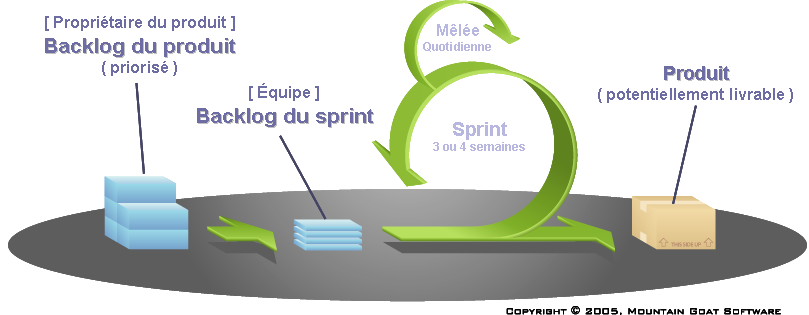
\includegraphics[width=\linewidth]{Images/scrum.png}
  \caption{Processus scrum}
  \label{fig:scrum}
\end{figure}
La planification du sprint correspond à lister les points prioritaires que l'équipe
pense pouvoir réaliser au cours d'un sprint.\\[0.2cm]
La revue du sprint a lieu en fin de sprint, l'équipe de développement présente les
fonctionnalités terminées au cours du sprint et recueille les retours du représentant des
utilisateurs finaux, c'est aussi à ce moment que la mise en place des prochains sprints peut être
anticipée.\\[0.2cm]
La Rétrospective de Sprint permet de faire un point sur le sprint en lui-même (productivité, efficacité, qualité…) afin de pouvoir s'améliorer pour les prochains sprints.\\[0.2cm]
Enfin la mêlée quotidienne permet de faire un point sur les avancements de chacun,
elle est courte et chacun réponds à trois questions principales : Qu'est-ce que j'ai terminé
depuis la dernière mêlée ? Qu'est-ce que j'aurai terminé d'ici la prochaine mêlée ? Quels
obstacles me retardent ?
\subsection{L'équipe SCRUM}
L’équipe a un rôle capital dans SCRUM : elle est constituée dans le but d’optimiser la flexibilité et la productivité; pour cela, elle s’organise elle-même et doit avoir toutes les compétences nécessaires au développement du produit. Elle est investie avec le pouvoir et l’autorité pour faire ce qu’elle a à faire.\\[0.5cm]
Scrum definit les rôles suivants :
\begin{description}
\item[Le Product Owner (le propriétaire du produit) : ] c’est une personne qui porte la vision du produit à réaliser, généralement c’est un expert dans le domaine.
\item[Le SCRUM Master (le directeur de produit) : ]c'est la personne qui doit assurer le bon déroulement des différents sprints du release, et qui doit impérativement maitriser SCRUM. 
\item[Le SCRUM Team (l’équipe de SCRUM) : ] constitué des personnes qui seront chargées d’implémenter les différents besoins du client. Bien évidemment, cette équipe sera constituée des développeurs, des testeurs, etc.
\end{description}
Dans le contexte de notre projet, Mr RHANIZAR serait  le propriétaire du produit, et le directeur du produit puisqu’il satisfait les différents prés-requis de ces rôles cités précédemment et nous formons ELKAISSI SOUHAIL et CHATRIA ZAKARIA les deux membres de l’équipe SCRUM. 
\section{Langage de modélisation}
Le langage de modélisation adopté durent ce stage sera le UML ,comme étant un outil comportant multiples points forts notamment sa standardisation ainsi que les divers diagrammes qu’il propose, et qui permettent la schématisation des systèmes complexes sous un format graphique et textuel simplifié et normalisé.\\
Généralement, le recours à la modélisation UML et plus particulièrement UML 2.0 procure de nombreux avantages qui agissent sur :
\begin{itemize}
\item La modularité.
\item L’abstraction.
\item La dissimulation.
\item La structuration cohérente des fonctionnalités et des données.
\end{itemize}
\section{TensorFlow : Librairie du machine learining et deep learning}
TensorFlow est une bibliothèque de logiciels open source pour le calcul numérique utilisant des graphes de flux de données. Il a été initialement développé par l'équipe Google Brain au sein de l'organisation de recherche Machine Intelligence de Google pour l'apprentissage automatique et la recherche sur les réseaux neuronaux profonds, mais le système est assez général pour être applicable dans une grande variété d'autres domaines. Il a atteint la version 1.0 en février 2017 et a poursuivi son développement rapide, avec plus de 21 000 engagements à ce jour, dont un grand nombre de contributeurs externes.\\[0.5cm]
TensorFlow est multi-plateforme. Il fonctionne sur presque tout : les processeurs graphiques et les processeurs normaux, y compris les plates-formes mobiles et embarquées, et même les unités de traitement tensoriel (TPU), qui sont des matériels spécialisés pour faire des calculs tensoriels. Ils ne sont pas encore largement disponibles, mais nous avons récemment lancé un programme alpha.

\section{Planification prévisionnelle}
\begin{tabular}{|p{6cm}|p{3cm}|p{3cm}|p{2cm}|}
\hline
\textbf{Nom de la tâche} & \textbf{Début de la tache} & \textbf{Date de la fin} & \textbf{Durée} \\
\hline
 Début du stage cadre & 23/04/2018 & 23/04/2018 & 1j\\
\hline
 Phase de preparation & 23/04/2018 & 01/05/2018 & 5j\\
\hline 
\textit{\hspace{1cm}Étude de la Solution actuelle} & \textit{22/04/2018} &  \textit{24/04/2018} & \textit{2j}\\
\hline
\textit{\hspace{1cm}Compréhension la totalité du projet} & \textit{25/04/2018} & \textit{01/05/2018} &  \textit{3j}\\
\hline
\textbf{Sprint 1: }Réalisation d'un modèle de prédiction avec l'algorithme CNN & 02/05/2018 & 23/05/2018 & 18j\\
\hline
Rédaction du Rapport & 25/05/2018 & 25/05/2018 & 1j \\
\hline
\textbf{Sprint 2: }Réalisation d'un modèle de prédiction avec la méthode SVM & 25/05/2018 & 04/06/2018 & 7j\\
\hline
\textbf{Sprint 3: }Amélioration du modèle CNN en ajoutant une couche de word2vec & 05/06/2018 & 13/06/2018 & 8j\\

\hline 
\textbf{Sprint 4: }Réalisation d'un modèle hybride qui regroupe CNN avec word2vec et le SVM & 14/06/2018 & 06/07/2018 & 17j\\
\hline
Soutenance du Projet Cadre & 22/06/2018 & 22/06/2018 & 1j\\
\hline
\textbf{Sprint 5: }Déploiement de la solution & 09/07/2018 & 14/07/2018 & 5j\\
\hline
\end{tabular}
\begin{figure}[h]
  \caption{planification prévisionnelle}
  \label{fig:planification}
\end{figure}
